In questo capitolo verrà esplorata l'implementazione delle funzionalità chiave per il miglioramento della funzionalità di monitoraggio delle presenze di ZConnect. Nella Sezione 4.1, sarà analizzato l'algoritmo appositamente progettato per determinare la porzione di mappa da visualizzare quando l'utente apre la mappa, con l'obiettivo di fornire una chiara visualizzazione della posizione dell'utente e dell'area di lavoro più vicina. Verrà introdotto, nella Sezione 4.2, l'algoritmo utilizzato per calcolare la distanza tra la posizione dell'utente e il bordo più prossimo del geofence. Successivamente, nella Sezione 4.3, verrà esplorata l'implementazione della funzionalità ``follow-me", focalizzandosi su come questa caratteristica agevoli l'utente a raggiungere il luogo di lavoro preposto avendo il supporto della mappa. Infine, nella Sezione 4.4, verrà affrontato il tema della prevenzione della falsificazione della posizione nell'ambiente iOS di ZConnect, evidenziando le scelte implementative adottate.

\section{Determinare la porzione di mappa da visualizzare}
Un aspetto critico per il miglioramento della funzionalità di monitoraggio delle presenze di ZConnect, come visto nella Sezione \ref{Progettazione}, è quello di fornire all'utente, all'apertura della mappa, una visuale esaustiva della sua posizione e dell'area di lavoro a lui più vicina.

Per fare questo è stato necessario definire un algoritmo, chiamato zoomToUserAndGeoFence, a cui, passata la posizione dell'utente ed il geofence a lui più vicino, mostri la porzione di mappa corretta, che comprenda la posizione dell'utente ed il centro del geofence più vicino.
La determinazione del geofence più vicino all'utente verrà approfondita nella Sezione 4.2.

\begin{lstlisting}[
    basicstyle=\footnotesize, language = Java %or \small or \footnotesize etc.
]
void zoomToUserAndGeoFence(IGeoPoint geoPoint, GeoFenceWithDistance geoFence);
\end{lstlisting}

Come già analizzato, le versioni Android e iOS di ZConnect utilizzano librerie diverse per visualizzare la mappa. La versione Android di ZConnect utilizza la libreria Osmdroid.

La libreria Osmdroid tra i vari metodi e classi fornisce la classe BoundingBox \cite{BoundingBox}, che definisce una porzione di mappa tramite quattro coordinate geografiche: nord, sud, est ed ovest, modellate come float. Questa classe risulta quindi essenziale per poter definire la porzione di mappa da visualizzare. Di conseguenza per definire la porzione di mappa da visualizzare è stato imperativo definire i quattro vertici della BoundingBox.

Per fare questo, inizialmente è stato necessario calcolare il raggio della BoundingBox, ovvero il raggio della porzione di mappa da visualizzare. \'E stato scelto come raggio la distanza tra la posizione dell'utente ed il centro del geofence, il cui calcolo verrà illustrato in seguito, per avere la certezza che nella porzione di mappa scelta fosse sempre compresa la posizione dell'utente ed il centro del geofence a lui più vicino.

I vertici della BoundingBox sono però modellati come gradi di latitudine e longitudine, si è quindi reso necessario convertire la distanza, espressa in metri, in gradi di latitudine e longitudine. 
Per ottenere questo risultato sono state usate delle approssimazioni, in particolare si è considerato che $111111$ metri sono $1$ grado di latitudine e che $\frac{\text{distanza}}{ 111111 \cdot \cos{\text{\{latitudine\}}}} $ è un grado di longitudine.

Quindi ipotizzando che al metodo zoomToUserAndGeoFence siano passati i seguenti dati, che rappresentano le coordinate della posizione dell'utente e le coordinate del geofence:

\begin{lstlisting}[
    basicstyle=\footnotesize, language = Java %or \small or \footnotesize etc.
]
geoPoint.getLatitude = 44.87
geoPoint.getLongitude = 010.21

geoFence.getMaxLatitude = 44.86
geoFence.getMaxLongitude = 10.28
geoFence.getMinLatitude = 44.86
geoFence.getMinLongitude = 10.27

geoFence.getDistanceToCenter = 5154.18 metri
\end{lstlisting}

vengono calcolati i gradi di latitudine e longitudine della distanza tra la posizione dell'utente ed il centro del geofence con le approssimazioni precedentemente illustrate:

\[\begin{split}
    &\text{longitudeBoundingBoxRadious} = | \frac{5154.18}{111111} | = 0.046 \\
    &\text{latitudeBoundingBoxRadious} = | \frac{5151.18}{\cos{44.87 \cdot 111111}} | = 0.06
\end{split}\]

Dopo aver calcolato i gradi di latitudine e longitudine corrispondenti alla distanza tra l'utente ed il centro del geofence a lui più vicino sono stati determinati i vertici della BoundingBox trovando i punti più a Nord, Est, Sud e Ovest.
Per determinare questi punti è stato scelto come punto centrale della BoundingBox la posizione dell'utente, rendendo così necessario sommare e sottrarre opportunamente la latitudine e la longitudine della distanza tra la posizione dell'utente ed il centro del geofence con la latitudine e longitudine della posizione dell'utente.
Per determinare il punto più a Nord è stata sommata la latitudine della posizione dell'utente con la latitudine della distanza tra l'utente ed il centro del geofence. Per determinare il punto più a Est è stata sottratta la longitudine della distanza tra l'utente ed il centro del geofence alla longitudine della posizione dell'utente. Per determinare il punto più a sud è stata sottratta la latitudine della distanza tra l'utente ed il centro del geofence alla latitudine della posizione dell'utente. Infine per determinare il punto più ad ovest è stata sommata la longitudine della posizione dell'utente con la longitudine della distanza tra l'utente ed il centro del geofence.
Così facendo è stata determinata la porzione di mappa da mostrare.

Con i dati precedenti si otterrebbero i seguenti vertici:

\[\begin{split}
    &\text{Nord}: 44.87 + 0.06 = 44.93 \\
    &\text{Est}: 010.21 - 0.046 = 010.16 \\
    &\text{Sud}: 44.87 - 0.06 = 44.81 \\
    &\text{Ovest}: 010.21 + 0.046 = 010.26 \\
\end{split}\]

Nella versione iOS di ZConnect per definire la porzione di mappa da visualizzare è stata utilizzata la classe MKPolygon \cite{MKPolygon}, la quale permette di definire un poligono passando come argomenti del costruttore una lista di vertici modellati come latitudini e longitudini. \' E stato necessario anche per la versione iOS calcolare i quattro vertici del MKPolygon per determinare la porzione di mappa da visualizzare. Per fare questo sono stati eseguiti gli stessi passaggi illustrati in precedenza per la versione Android di ZConnect.

Con i dati di esempio precedente si ottiene la porzione di mappa in Figura \ref{fig:porzione_mappa}.

\begin{figure}[ht!]
    \centering
    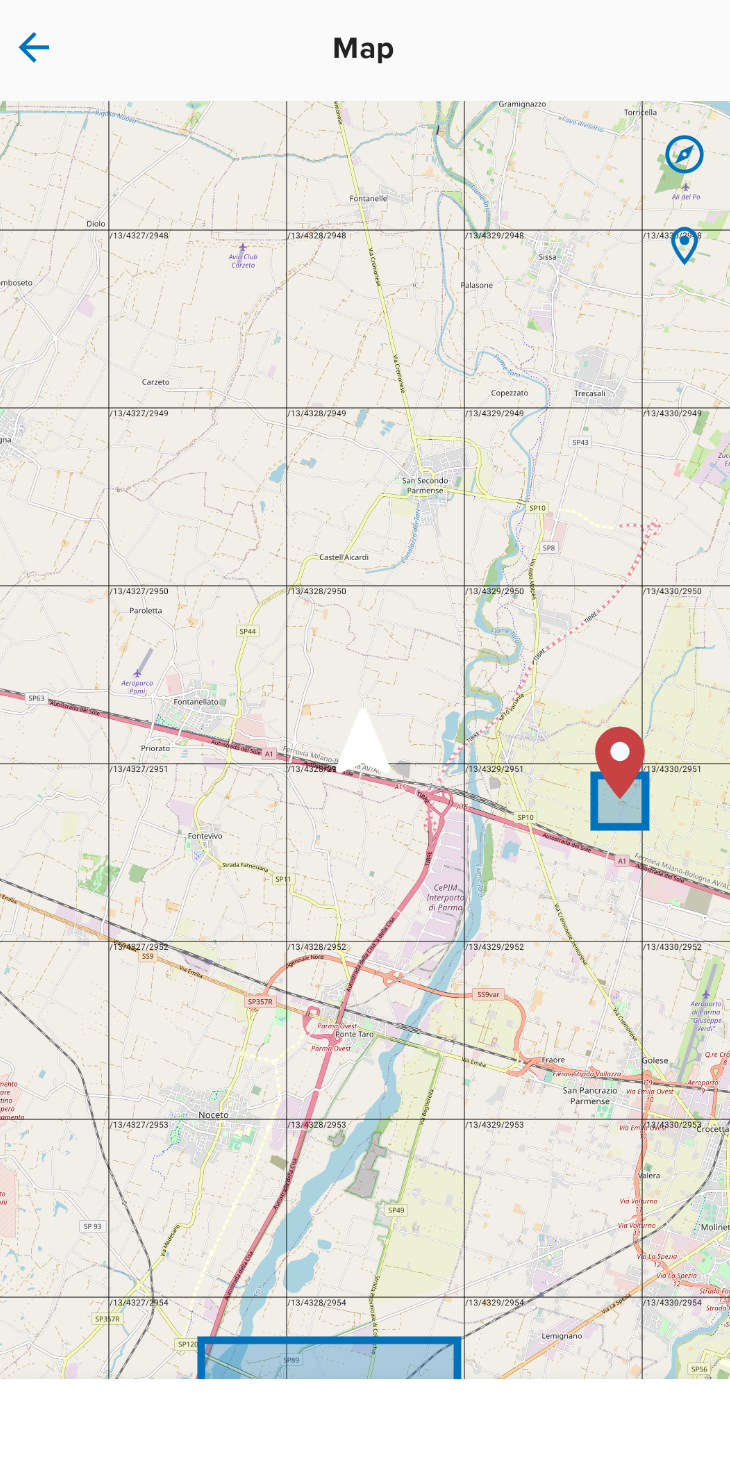
\includegraphics[width=0.4\textwidth]{Immagini/zoom_dati_esempio.png}
    \caption{Porzione di mappa ottenuta nella Sezione 4.1}
    \label{fig:porzione_mappa}
\end{figure}

\section{Distanza dal bordo del geofence}
Per determinare la porzione di mappa da mostrare è stato necessario stabilire quale fosse il luogo di lavoro più vicino all'utente nel momento in cui apre la mappa. Per stabilire quale luogo di lavoro fosse più vicino all'utente, dato che, come già visto, ad un utente è associata una lista di luoghi di lavoro, si è scelto di ordinare la lista dei luoghi di lavoro associata all'utente in base alla distanza tra il luogo di lavoro e l'utente, per poi scegliere il luogo di lavoro con distanza minore. In queste Sezione verrà trattato l'algoritmo per calcolare la distanza tra la posizione dell'utente ed un luogo di lavoro.

Come approfondito nella Sezione \ref{Analisi_sistema}, un area di lavoro è modellata come un istanza della classe GeoFence. Tutti i geofence utilizzati sono di tipo quadrato e sono definiti da quattro properties che servono ad identificare i vertici del quadrato, ovvero le latitudini e longitudini massime e minime. Inoltre ogni geofence ha associato il suo centro, modellato come un istanza della classe GeoPoint, che è una classe creata per rappresentare all'interno di ZConnect delle posizioni di punti sulla superficie terrestre, infatti ogni GeoPoint è identificato dalla sua latitudine e longitudine.

Date queste caratteristiche, per stabilire quale sia il geofence più vicino all'utente è necessario stabilire, per ogni geofence associato all'utente, la distanza tra la posizione dell'utente ed il bordo del geofence più prossimo. \'E fondamentale anche calcolare la distanza tra la posizione dell'utente ed il centro del geofence, poiché in caso di due o più geofence con distanza tra l'utente ed il bordo più prossimo uguale, viene considerato come geofence più vicino quello con distanza tra la posizione dell'utente ed il centro minore.

\subsection{Determinare il bordo più vicino}
Per calcolare la distanza tra la posizione dell'utente ed il bordo del geofence più prossimo all'utente è necessario prima stabilire qual'è il bordo del geofence più vicino all'utente, evitando così di calcolare la distanza tra la posizione dell'utente ed ogni bordo del geofence per poi selezionare la distanza minore.

Nella classe GeoFence è stato creato un metodo, calculateDistanceToBorder, che prende come argomento un GeoPoint e restituisce la distanza tra il punto passato come argomento e il bordo più vicino al GeoFence stesso. Per determinare quale sia il bordo del geofence più vicino alla posizione passata sono stati inizialmente identificati i quattro vertici del geofence, è stato possibile farlo perchè il geofence ha come properties le latitudini e longitudini massime e minime. Quindi i vertici del geofence sono modellati come GeoPoint risultanti dal prodotto cartesiano tra le latitudini e le longitudini del geofence.
Ad esempio se le properties del geofence sono i seguenti:
\begin{lstlisting}[
    basicstyle=\footnotesize, language = Java %or \small or \footnotesize etc.
]
maxLatitude = 44.77
maxLongitude = 10.23
minLatitude = 44.72
minLongitude = 10.17
\end{lstlisting}

i vertici dei geofence verranno composti in questo modo:

\begin{lstlisting}[
    basicstyle=\footnotesize, language = Java %or \small or \footnotesize etc.
]
GeoPoint top_right_vertex = new GeoPoint(maxLatitude, maxLongitude);
GeoPoint top_left_vertex = new GeoPoint(maxLatitude, minLongitude);
GeoPoint bottom_left_vertex = new GeoPoint(minLatitude, minLongitude);
GeoPoint bottom_right_vertex = new GeoPoint(minLatitude, maxLongitude);
\end{lstlisting}

Dopo aver identificato i vertici del geofence, si è deciso, immaginando di posizionare il geofence su un piano cartesiano, che rappresenta la superficie terrestre, di dividere lo spazio in settori; proiettando verso più e meno infinito le latitudini e longitudini massime e minime del geofence. Così facendo si vengono a creare nove settori. Come si può vedere nella tabella \ref{tab:settori} i settori sono stati numerati sequenzialmente, partendo dal settore in alto a sinistra. Seguendo questa numerazione il settore cinque è quello che rappresenta l'area del geofence.

\begin{table}[ht!]
    \centering
    \begin{tabular}{c|c|c}
       1 & 2 & 3 \\
       \hline
       4 & 5 & 6 \\
    \hline
       7 & 8 & 9
    \end{tabular}
    \caption{Divisione dello spazio in settori}
    \label{tab:settori}
\end{table}

Una volta identificati questi settori, confrontando la latitudine e la longitudine della posizione dell'utente con la latitudine e longitudine dei vertici del geofence, è possibile stabilire in che quadrante è posizionato l'utente.
Ad esempio se la posizione dell'utente, che è passata come argomento al metodo calculateDistanceToBorder, ha la seguente latitudine e longitudine:
\begin{lstlisting}[
    basicstyle=\footnotesize, language = Java %or \small or \footnotesize etc.
]
point_latitude = 37.42
point_longitude = -122.08
\end{lstlisting}

Confrontando la latitudine e la longitudine della posizione dell'utente con le latitudini e longitudini minime e massime del geofence, si stabilisce che la posizione dell'utente cade nel settimo settore, in quanto la latitudine della posizione dell'utente è minore uguale della latitudine minima del geofence e la longitudine della posizione dell'utente è minore uguale della longitudine minima del geofence.

Una volta identificato qual'è il settore in cui è contenuta la posizione dell'utente si è stabilito anche qual'è il bordo più vicino all'utente, in quanto è sempre il bordo che fa parte del settore identificato.
Nei casi in cui la posizione dell'utente sia contenuta nei quadranti 1, 3, 7 e 9, non viene identificato il bordo del geofence, ma viene identificato un vertice, in quanto, per qualsiasi posizione all'interno di questi quadranti, la distanza minima tra quella posizione ed il geofence sarà sempre la distanza tra quella posizione ed il vertice contenuto nel quadrante identificato. 
Nell'esempio precedente quindi viene identificato come bordo più vicino il vertice bottom\_left\_vertex.

\subsection{Calcolo della distanza dal bordo}
Grazie all'algoritmo precedentemente illustrato è stato possibile identificare quale fosse il bordo del geofence più vicino all'utente. Avendo identificato il bordo più vicino, modellato tramite i due vertici che lo compongono, che a loro volta sono modellati tramite istanze della classe GeoPoint, è stato possibile calcolare la distanza minima tra la posizione dell'utente ed il bordo identificato come quello più vicino all'utente.

Come visto in precedenza, si può identificare come bordo più vicino un segmento o un punto. Nel caso in cui venga identificato un punto è necessario calcolare la distanza tra due punti, la posizione dell'utente e il vertice del geofence identificato come quello più vicino all'utente. Per raggiungere questo obiettivo è stato implementato un metodo nella classe GeoPoint, getHaversineDistance:
\begin{lstlisting}[
    basicstyle=\footnotesize, language = Java %or \small or \footnotesize etc.
]
/**
* Computes the minimum distance between current geopoint and a second 
* geopont using the Haversione Formula
* @param from The geopoint from which to compute distance
* @return The distance
*/
double getHaversineDistance(IGeoPoint from);
\end{lstlisting}

che permette di calcolare la distanza tra la posizione dell'utente, modellata tramite un'istanza della classe GeoPoint, ed una seconda posizione, passata come argomento del metodo stesso, utilizzando la formula di Haversine. La formula di Haversine determina la distanza tra due punti su una sfera, date le loro longitudini e latitudini.
Viene riportata di seguito la formula di Haversine, dove $\phi$ è la latitudine, $\lambda$ è la longitudine e $R$ è il raggio della terra:

\begin{align*}
a & = \sin^2\left(\frac{\phi_2 - \phi_1}{2}\right) + \cos\phi_1 \cdot \cos\phi_2 \cdot \sin^2\left(\frac{\lambda_2 - \lambda_1}{2}\right) \\
c & = 2 \cdot \mathrm{atan2}\left(\sqrt{a}, \sqrt{1-a}\right) \\
d & = R \cdot c
\end{align*}

Invece, nel caso in cui venga identificato un segmento è necessario calcolare la distanza minima tra un punto ed un segmento. Per fare questo è stato implementato un altro metodo nella classe GeoPoint, getMinimumDistancePointLine:

\begin{lstlisting}[
    basicstyle=\footnotesize, language = Java %or \small or \footnotesize etc.
]
/**
* Computer the distance bewteen two given geopoint and a third geopoint
*
* @param vertex1
* @param vertex2
* @return
*/
double getMinimumDistancePointLine(IGeoPoint vertex1, IGeoPoint vertex2);
\end{lstlisting}

che permette di calcolare la distanza tra la posizione, modellata tramite l'istanza della classe GeoPoint, ed un segmento, modellato tramite i suoi due vertici, passati come argomento al metodo stesso.
Innanzitutto è stato calcolato l'angolo di Bearing assoluto dei due segmenti formati dai vertici del bordo più vicino e la posizione dell'utente. L'angolo di Bearing è l'angolo formato tra il segmento ed il nord magnetico.
Considerando la posizione dell'utente come punto A ed i vertici del segmento come punti B e C, il calcolo dell'angolo di Bearing è il seguente, dove $\phi$ è la latitudine, $\lambda$ è la longitudine e $R$ è il raggio della terra:

\begin{align*}
\text{bearingAC} & = \mathrm{atan2}\left( \sin(\lambda_C - \lambda_A) \cdot \cos(\phi_2), \cos(\phi_1) \cdot \sin(\phi_2) - \sin(\phi_1) \cdot \cos(\phi_2) \cdot \cos(\phi_C - \phi_A) \right) \\
\text{bearingAB} & = \mathrm{atan2}\left( \sin(\lambda_B - \lambda_A) \cdot \cos(\phi_2), \cos(\phi_1) \cdot \sin(\phi_2) - \sin(\phi_1) \cdot \cos(\phi_2) \cdot \cos(\phi_B - \phi_A) \right)
\end{align*}

Gli angoli di Bearing ottenuti sono stati normalizzati, in modo da ottenere valori compresi tra 0 e 360.
Successivamente è stata calcolata la distanza tra il punto A ed il punto C utilizzando la formula di Haversine, precedentemente illustrata.
Infine è stata calcolata la cross-track distance, ovvero la distanza tra un punto ed un segmento su una sfera, distanza chiamata great circle path.
La formula per calcolare la cross-track distance è la seguente:

\begin{align*}
d_{xt} = \sin^{-1}\left( \sin(\delta_{13}) \cdot \sin(\theta_{13} - \theta_{12}) \right) \cdot R
\end{align*}

dove:
\begin{itemize}
    \item $\delta_{13}$ è la distanza tra il punto di partenza ed il terzo punto. Nell'esempio precedente è la distanza tra A e C
    \item $\theta_{13}$ è l'angolo di Bearing tra il punto di partenza ed il terzo punto. Nell'esempio precedente è l'angolo di Bearing del segmento AC.
    \item $\theta_{12}$ è l'angolo di Bearing tra il punto di partenza ed il secondo punto. Nell'esempio precedente è l'angolo di Bearing del segmento AB.
    \item $R$ è il raggio della terra.
\end{itemize}

Grazie a questo algoritmo viene calcolata la distanza tra la posizione dell'utente ed il bordo del geofence che permette di selezionare il geofence più vicino all'utente nel momento in cui apre la mappa.

\section{Follow-me}
Per migliorare la funzionalità di monitoraggio delle presenze di ZConnect in questo lavoro di tesi è stato deciso di implementare la funzionalità del ``follow-me", come approfondito nella Sezione \ref{Progettazione}. Questa funzionalità facilita l'utente nel raggiungimento dell'area di lavoro poiché, una volta attivata, il marker che rappresenta la posizione dell'utente rimane al centro della schermata della mappa durante gli spostamenti dell'utente.

Anche in questo caso, a causa del duplice sviluppo di ZConnect per Android l'implementazione di questa funzionalità cambia notevolmente tra i due sistemi operativi.

Come già detto la versione Android di ZConnect utilizza la libreria Osmdroid \cite{OpenStreetMapWiki} per la visualizzazione e l'interazione con la mappa. La libreria Osmdroid fornisce una classe, MyLocationNewOverlay \cite{MyLocationNewOverlay}, che permette di rappresentare la posizione del device sulla mappa tramite un marker. La classe MyLocationNewOverlay ha associato un LocationProvider \cite{LocationProvider}, passato come argomento nel costruttore, grazie al quale è in grado di conoscere la posizione del device e reagire agli spostamenti, ridisegnando il marker sulla mappa. Inoltre la classe MyLocationNewOverlay espone i metodi enableFollowLocation e disableFollowLocation, i quali permettono di abilitare la funzionalità ``follow-me" che permette di centrare la mappa sulla posizione corrente del MyLocationNewOverlay e automaticamente spostarla quando viene rilevato un cambio di posizione, in modo da far rimanere sempre al centro della mappa il marker che rappresenta la posizione del dispositivo.

Quindi per implementare la funzionalità di ``follow-me" nella versione Android è bastato utilizzare come marker per la posizione dell'utente un istanza della classe MyLocationNewOverlay ed utilizzare i suoi metodi per attivare e disattivare la funzionalità, la quale viene poi gestita in automatico dalla libreria Osmdroid.

A differenza di Android, la versione iOS di ZConnect utilizza la libreria MapKit \cite{MapKitDoc} che è fornita direttamente da Apple.
La libreria MapKit fornisce la classe MKMapView usata per mostrare ed interagire con la mappa \cite{MKMapView}. La libreria MKMapView implementa dei metodi per mostrare e manipolare dei contenuti sulla mappa. Per mostrare la posizione del device sulla mappa è stato utilizzato il metodo showUserLocation della classe MKMapView. Attivando questa funzione viene visualizzato sulla mappa un marker blu in corrispondenza della posizione del device. Il marker reagisce anche allo spostamento del device ridisegnandosi in corrispondenza della nuova posizione rilevata.

La libreria MapKit non fornisce, a differenza di Osmdroid, la funzionalità ``follow-me" integrata nella classe che rappresenta il marker dell'utente. Quindi per implementare la funzionalità di ``follow-me" è stata usata la classe MKMapCamera \cite{MKMapCamera} fornita anch'essa dalla libreria MKMapKit. Un'istanza di questa classe definisce un punto di vista virtuale sopra la superficie della mappa e influenza il modo in cui MapKit presenta la mappa all'utente.

La classe MKMapView fornisce una funzione di call-back che viene chiamata dal sistema operativo quando la posizione del device cambia, in questa funzione viene controllato se l'utente ha attivato funzionalità di ``follow-me", se è attiva viene settata la property centerCoordinate, della classe MKMapCamera, con le coordinate prese dalla posizione dell'utente, che la classe MKMapView salva nella variabile userLocation. Dopo aver settato le coordinate del centro della mappa, tramite la funzione setCamera della classe MKMapView viene animata la mappa per essere centrata sulla nuova posizione dell'utente.

Così facendo è stata implementata la funzionalità di ``follow-me" in iOS, agevolando anche gli utenti della versione iOS di ZConnect nel raggiungimento dell'area di lavoro.

\section{Fake position iOS}
Nel capitolo di Analisi si era identificato come caratteristica dell'applicazione la prevenzione di possibili falsificazioni della posizione del dispositivo da parte dell'utente, in modo da evitare che l'utente possa registrare la propria presenza sul posto di lavoro anche quando non è fisicamente lì.
Questo controllo sulla falsificazione della posizione dell'utente nella versione iOS di ZConnect non era stato implementato prima di questo lavoro di tesi, a differenza della versione Android di ZConnect che controllava anche prima di questo lavoro di tesi la veridicità della posizione dell'utente.

Quindi è stato necessario implementare un controllo sulla eventuale falsificazione della posizione dell'utente nella versione iOS di ZConnect.

La classe che si occupa di implementare la classe che in iOS si occupa di rilevalre la posizione dell'utente è LocationManager. La classe che in iOS si occupa di rilevare la posizione del device è CLLocationManager. Il CLLocationManager è il luogo centrale per gestire i comportamenti legati alla posizione dell'applicazione. Si può utilizzare un oggetto location-manager per configurare, avviare e interrompere i servizi di localizzazione \cite{CLLocationManager}.

Nella classe LocationManager è stato creato un metodo, isMockLocation, per identificare se la posizione rilevata dal CLLocationManager è fittizia oppure deriva dalla vera posizione del device. Per raggiungere questo obiettivo sono stati usati i metodi isSimulatedBySoftware e isProducedByAccessory della classe CLLocationSourceInformation. La classe CLLocationSourceInformation contiene informazioni sulla fonte che fornisce un'istanza di CLLocation \cite{CLLocationSourceInformation}. Un oggetto CLLocation contiene la posizione geografica e l'altitudine di un dispositivo, insieme a valori che indicano l'accuratezza di tali misurazioni e il momento in cui sono state raccolte \cite{CLLocation}.
Il metodo isSimulatedBySoftware restituisce un valore booleano che indica se la posizione rilevate è stata generata da un software come Xcode, mentre il metodo isProducedByAccessory restituisce un valore booleano che indica se la posizione è stata generata da un accessorio esterno.

Il metodo isMockLocation, implementato nella classe LocationManager, controlla i risultati dei metodi isSimulatedBySoftware e isProducedByAccessory. Se uno dei due risultati è vero allora la posizione rilevata dal CLLocationManager è stata falsificata dall'utente.

Ora, per verificare se una posizione è stata falsificata, è necessario invocare il metodo isMockLocation dall'istanza della classe LocationManager, utilizzata per ottenere la posizione del dispositivo. Questo metodo esegue un controllo per determinare se la posizione ricevuta dal CLLocationManager è di natura simulata o rappresenta effettivamente la reale posizione del dispositivo.